%%
%% SEMANTiCS 2026 -- Posters & Demos track submission
%% Alternative draft: mirrors the structure of
%% Braun & Käfer, "Attribute-based Access Control on Solid Pods
%% using Privacy-friendly Credentials" (SEMANTiCS 2022).
%% CEUR-ART single-column, 5 pages incl. references.
%%
\documentclass[sigconf,natbib=true]{ceurart}

\usepackage{hyperref}

\usepackage{tikz}
\usetikzlibrary{shapes.geometric, arrows.meta, positioning, calc, backgrounds, fit, shadows, shapes.misc}

\definecolor{arrowcol}{HTML}{5D6D7E}
\definecolor{boxgray}{RGB}{80, 80, 90}
\definecolor{phasebg1}{RGB}{230, 240, 250}
\definecolor{phasebg2}{RGB}{255, 250, 235}
\definecolor{phasebg3}{RGB}{255, 240, 245}

\begin{document}

\copyrightyear{2026}
\copyrightclause{Copyright for this paper by its authors.
  Use permitted under Creative Commons License Attribution 4.0
  International (CC BY 4.0).}

\conference{SEMANTiCS 2026: 22nd International Conference on Semantic Systems,
  September 15--17, 2026, Ghent, Belgium}

\title{AMA-KBQA: A Multi-Agent Demo for Generalisable Question Answering over Heterogeneous Knowledge Graphs}

\author[1]{Yannic Duan}[email=uyfnw@student.kit.edu]
\author[1]{Maurice Bardenhagen}[email=uhyaa@student.kit.edu]
\author[1]{Maximilian Klattig}[email=ulumu@student.kit.edu]
\author[1]{Yuyang Li}[email=yuyang.li@kit.edu]
\address[1]{Institute AIFB, Karlsruhe Institute of Technology (KIT), Kaiserstr.\ 12, 76131 Karlsruhe, Germany}

\begin{abstract}
Our demo showcases AMA-KBQA, a multi-agent system that answers natural
language questions against structurally different RDF knowledge graphs
through a single, training-free reasoning core. A user at the booth
can ask both encyclopaedic questions, served from a Wikidata-derived
graph, and scholarly questions, served from the Open Research
Knowledge Graph. Each step of the agent's reasoning is exposed through
a web interface: question classification, tool calls over SPARQL and
vector search, scratchpad state, and final answer synthesis. The
system requires no fine-tuning, since onboarding a new knowledge graph
reduces to writing thin SPARQL wrappers behind an abstract tool
interface exposed via the Model Context Protocol.
\end{abstract}

\begin{keywords}
  KBQA \sep
  SPARQL \sep
  Large Language Models \sep
  Model Context Protocol \sep
  Multi-Agent Systems
\end{keywords}

\maketitle

%% ---------------------------------------------------------------
\section{Introduction}

Large language models (LLMs) increasingly serve as natural-language
front-ends to structured data, but on their own they suffer from
knowledge cutoff, hallucination, and brittle multi-hop
reasoning~\cite{ji2023survey}. Knowledge Base Question Answering
(KBQA) over RDF graphs mitigates these issues by grounding answers in
verifiable facts, but existing systems are typically engineered for
one specific graph and frequently rely on dataset-specific
fine-tuning. Both forms of coupling are costly: porting a system to a
new graph means rewriting the pipeline, and adopting a stronger LLM
means re-training.

This rigidity is particularly painful in corporate settings, where the
underlying knowledge graphs evolve continuously: new domains are
onboarded, schemas are refactored, and entire data sources are added,
replaced, or deprecated as business needs change. A KBQA system that
must be re-engineered or retrained for every such change is
impractical to operate. What is needed instead is a framework that
treats both the knowledge graph and the language model as swappable
components, so that adapting to a new data source or a stronger model
is a matter of configuration rather than re-implementation.

Our demo showcases \textbf{AMA-KBQA}, a multi-agent KBQA system whose
reasoning core is decoupled from both the underlying RDF graph and the
specific LLM driving it. A visitor to our booth can:
\begin{itemize}
  \item ask natural-language questions through a web interface against
        two structurally different knowledge graphs,
  \item see the same reasoning core answer both encyclopaedic and
        scholarly questions without any change in configuration.
\end{itemize}

This paper is structured as follows. First, we discuss related work
on KBQA, agentic LLM systems, and tool protocols. We then walk
through the demo as a visitor would experience it. Hereafter, we
discuss the current system architecture and outline directions for
future work.

\section{Discussion of Related Work}

We briefly survey related work on KBQA over RDF graphs, agent-based
LLM systems, and tool-use protocols.

Classical KBQA approaches rely on semantic parsing of natural-language
questions into SPARQL or other formal queries~\cite{berant2013semantic};
retrieval-augmented generation pipelines~\cite{lewis2020retrieval}
combine LLM generation with retrieved evidence. Both lines of work
have produced strong results on individual benchmarks but tend to bind
the resulting system tightly to the schema, vocabulary, and tool surface
of a single knowledge graph, and many systems additionally depend on
dataset-specific fine-tuning of the underlying model. The KQAPro
benchmark~\cite{cao2022kqapro} captures this Wikidata-style factoid
setting, while SciQA~\cite{sciqa2023} targets scholarly questions over
the Open Research Knowledge Graph (ORKG); systems published against
these two benchmarks are typically distinct codebases.

The shift from monolithic prompt-based systems to agentic loops
follows the ReAct paradigm~\cite{yao2023react}, in which an LLM
interleaves reasoning steps with tool calls. Interactive-KBQA
re-frames KBQA itself as a multi-turn control loop over atomic graph
APIs~\cite{xiong-etal-2024-interactive}. Our work inherits this
agentic stance but couples it with deterministic pre-processing for
question classification and a configuration-driven adapter layer for
portability across knowledge graphs. In contrast to systems that
rely on fine-tuning the backbone LLM, our reasoning core is
training-free and inherits capability gains from each new generation
of general-purpose models simply by swapping the backbone.

Our journal-based agent workspace continues the line of
\emph{scratchpad} mechanisms first introduced for
intermediate-computation LLMs by Nye et al.~\cite{nye2021scratchpad}
and adapted into the Thought/Action/Observation loop of tool-using
agents by ReAct~\cite{yao2023react}. Our Lessons-Learned loop, which
distils LLM-judged reasoning traces into reusable few-shot examples
indexed by question type, continues the trajectory-as-exemplar
lineage of Synapse~\cite{zheng2024synapse} and the persistent
self-curated memory of Dynamic Cheatsheet~\cite{suzgun2025dynamic}.
Concurrent work on Agentic Context Engineering~\cite{zhang2025ace}
pushes the same direction toward a structured
Generator/Reflector/Curator decomposition, which our current pipeline
does not yet replicate.

For tool communication, we rely on the Model Context Protocol
(MCP)~\cite{anthropic2024mcp}, a recent open protocol for connecting
LLM-driven clients to typed tool servers. Using MCP separates the
reasoning core from the implementation of any specific graph tool and
turns access policy into a single, auditable boundary. Agents see
only the tools their MCP server exposes, and the wrappers themselves
can inject named-graph filters or row-level predicates before any
query reaches the triple store.

\section{Basic Demo Walkthrough}

A visitor interacts with AMA-KBQA through a multi-page web
application. Our PWA-style frontend, the agent backend, and the two
knowledge-graph back-ends are deployed on a single virtual machine and
served over the public Web.

On the \emph{Chat} page, the visitor selects an agent (either one of
the two graph-specific sub-agents or the orchestrator) and asks a
question in natural language. The orchestrator classifies the question
and dispatches it to one or more sub-agents; each sub-agent runs the
same three-phase lifecycle: a deterministic pre-processing step that
classifies the question type and extracts candidate entities, an
iterative tool-calling loop that explores the knowledge graph through
typed MCP tools and records its findings in a structured scratchpad,
and a final synthesis step that drafts the answer solely from the
scratchpad's verified facts. The answer is returned together with a
token-usage summary and links into two inspection views.

The \emph{Trace Inspector} renders the agent's run as a hierarchical
tree of spans, including question classification, individual LLM
calls, every tool invocation, and the final synthesis, with the raw
arguments and results of each step. The \emph{Graph View} renders the
subgraph the agent discovered during exploration as an interactive
network, with a scrubber that replays the snapshot taken after each
tool call that mutated the scratchpad. Together, the two views let
visitors see not only \emph{what} the system answered but \emph{why}
it answered that way, and at which step a wrong answer first went off
track.

To showcase forward-compatibility, the \emph{Settings} page lets the
visitor swap the backbone LLM between questions. The same reasoning
core, prompts, and adapters then run against a different model, and
the trace inspector exposes how the choice affects both reasoning
shape and answer quality.

For the review period, a working prototype is hosted publicly so that
reviewers can interact with the system end-to-end without any local
setup; it is available at \url{https://TODO-prototype-link}.
Source code and setup instructions will also be provided.

\section{Discussion of System Architecture}

With the current architecture we aim to provide a flexible, fully
training-free prototype rather than a production-tuned KBQA service.

The system is organised into three layers. An \emph{Agent Layer}
hosts a base reasoning core together with knowledge-graph-specific
sub-agents; the sub-agents inherit the core's classification, tool
loop, scratchpad, and synthesis logic and only override what is
genuinely graph-specific, such as the question typology and the
extraction of candidate entities. An \emph{MCP Layer} exposes typed
tools for entity discovery, schema introspection, graph navigation,
deterministic verification, and raw SPARQL; these tools are the only
way the agent ever touches the data. A \emph{Data Layer} pairs a
triple store for exact graph access with a vector store for fuzzy
entity and relation search.

Each sub-agent runs the same three-phase lifecycle
(Fig.~\ref{fig:agent_flow}): a pre-agent hook that classifies the
question and injects type-specific guidance, an iterative
tool-calling loop backed by a structured scratchpad of visited nodes,
discovered values, and verified facts, and a post-agent synthesis step
that drafts the final answer solely from the scratchpad. A loop
detector intervenes when the agent revisits the same tool or makes no
progress, and deterministic verification tools offload numeric and
boolean logic from the LLM.

\begin{figure}[t]
    \centering
    \resizebox{0.62\linewidth}{!}{%
    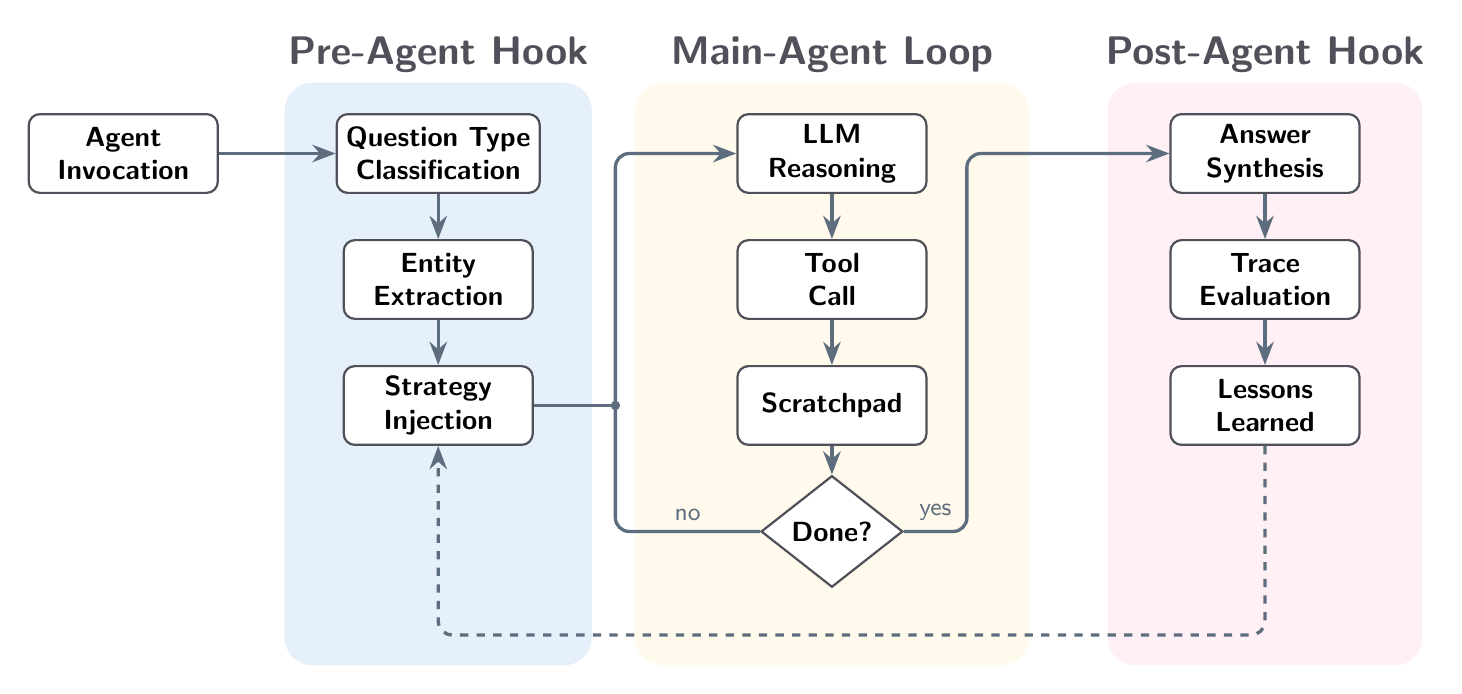
\begin{tikzpicture}[
        >=Stealth,
        %% Grid: y-rows at integer multiples of 1.6; x-columns at fixed centers.
        box/.style={rectangle, rounded corners=4pt, draw=boxgray, thick, fill=white, minimum width=2.4cm, minimum height=1.0cm, align=center, font=\sffamily\normalsize\bfseries},
        widebox/.style={box, minimum width=3.0cm},
        decision/.style={diamond, draw=boxgray, thick, fill=white, minimum width=1.8cm, minimum height=1.4cm, align=center, font=\sffamily\normalsize\bfseries, inner sep=1pt},
        arrow/.style={->, >=Stealth, line width=1.2pt, color=arrowcol, rounded corners=5pt},
        line/.style={color=arrowcol, line width=1.2pt, rounded corners=5pt},
        dasharrow/.style={->, >=Stealth, line width=1.2pt, dashed, color=arrowcol, rounded corners=5pt},
        phaselabel/.style={font=\sffamily\Large\bfseries, text=boxgray}
    ]
    %% --- Starting node (row y=3.2) ---
    \node[box] (user) at (-4.0, 3.2) {Agent\\Invocation};

    %% --- Pre-Agent Hook (top-aligned: rows 3.2, 1.6, 0) ---
    \node[box] (classifier) at (0,  3.2) {Question Type\\Classification};
    \node[box] (extractor)  at (0,  1.6) {Entity\\Extraction};
    \node[box] (strategy)   at (0,  0)   {Strategy\\Injection};

    %% --- Main-Agent Loop (rows 3.2, 1.6, 0, -1.6) ---
    \node[box]    (llm)      at (5.0,  3.2) {LLM\\Reasoning};
    \node[box]    (toolcall) at (5.0,  1.6) {Tool\\Call};
    \node[box]    (result)   at (5.0,  0)   {Scratchpad};
    \node[decision] (done)   at (5.0, -1.6) {Done?};

    %% --- Post-Agent Hook (top-aligned: rows 3.2, 1.6, 0) ---
    \node[box] (synthesis) at (10.5,  3.2) {Answer\\Synthesis};
    \node[box] (judge)     at (10.5,  1.6) {Trace\\Evaluation};
    \node[box] (lessons)   at (10.5,  0)   {Lessons\\Learned};

    %% --- Pre-Agent: sequential top-to-bottom ---
    \draw[arrow] (user.east) -- (classifier.west);
    \draw[arrow] (classifier.south) -- (extractor.north);
    \draw[arrow] (extractor.south)  -- (strategy.north);

    %% --- Shared entry into LLM.west: Done?-no + Strategy share the vertical at x=2.25 ---
    \draw[arrow] (done.west) -- (2.25, -1.6)
        node[midway, above, font=\sffamily\small] {no}
        -- (2.25, 3.2) -- (llm.west);
    \draw[line] (strategy.east) -- (2.25, 0);
    \node[circle, fill=arrowcol, inner sep=1.2pt] at (2.25, 0) {};

    %% --- Main loop internal: top-to-bottom ---
    \draw[arrow] (llm.south)      -- (toolcall.north);
    \draw[arrow] (toolcall.south) -- (result.north);
    \draw[arrow] (result.south)   -- (done.north);

    %% --- Done? "yes" exits east to Post-Agent Hook ---
    \draw[arrow] (done.east) -- ++(0.8, 0)
        node[midway, above, font=\sffamily\small] {yes}
        |- (synthesis.west);

    %% --- Post-Agent flow ---
    \draw[arrow] (synthesis.south) -- (judge.north);
    \draw[arrow] (judge.south)     -- (lessons.north);

    %% --- Feedback: Lessons Learned -> Strategy Injection (dashed, inside bgs, below Done?) ---
    \draw[dasharrow] (lessons.south) -- ++(0, -2.4) -| (strategy.south);

    %% --- Phase backgrounds + labels (compact: 7.4cm tall, centered to keep top headroom) ---
    \begin{scope}[on background layer]
        \node[rectangle, rounded corners=10pt, fill=phasebg1,
              minimum width=3.9cm, minimum height=7.4cm] at (0, 0.4) (bg1) {};
        \node[phaselabel, anchor=south] at (bg1.north) {Pre-Agent Hook};
        \node[rectangle, rounded corners=10pt, fill=phasebg2,
              minimum width=5.0cm, minimum height=7.4cm] at (5.0, 0.4) (bg2) {};
        \node[phaselabel, anchor=south] at (bg2.north) {Main-Agent Loop};
        \node[rectangle, rounded corners=10pt, fill=phasebg3,
              minimum width=4.0cm, minimum height=7.4cm] at (10.5, 0.4) (bg3) {};
        \node[phaselabel, anchor=south] at (bg3.north) {Post-Agent Hook};
    \end{scope}
    \end{tikzpicture}
    }
    \caption{Agent lifecycle: deterministic pre-processing, an iterative tool-calling main loop over a scratchpad, and post-hoc synthesis, trace evaluation, and lesson distillation.}
    \label{fig:agent_flow}
\end{figure}


Onboarding a new knowledge graph reduces to extending a base adapter
with URI prefixes, endpoints and vector collections, and providing
the abstract tools as SPARQL wrappers against the target endpoint. No
training data and no fine-tuning are required, and because every
sub-agent is a self-contained instance of the same template, the
architecture generalises naturally to a multi-agent setup in which an
orchestrator dispatches the question to relevant sub-agents and
merges their verified evidence into a single cross-source answer. To
decide which sub-agents to consult for a given query, the
orchestrator performs a lightweight vector search of the top entities
extracted from the question against each sub-agent's entity index and
invokes a sub-agent only when its index returns close matches, on the
assumption that the underlying graph then holds information about
those entities.

Because every interaction with a graph passes through deterministic
SPARQL wrappers exposed as MCP tools, access policy can be enforced
at a single auditable boundary rather than embedded in LLM prompts.
The set of MCP servers an agent is granted at runtime provides
coarse-grained control, while named-graph filters and row-level
predicates injected inside the wrappers themselves provide
fine-grained control. The LLM never authors raw access-control
logic and never sees forbidden triples.

To improve the system over time without retraining, we run a
\emph{Lessons-Learned} loop: high-quality reasoning traces are
distilled into reusable few-shot examples and tool tips, indexed by
question type, and re-injected into future runs. All generated
material is written to a shadow directory and reviewed before being
promoted to the live few-shot corpus, so the system can grow its own
guidance while keeping a human in the loop.

In an internal evaluation, the same reasoning core answered both
encyclopaedic factoid questions over the Wikidata-derived KQAPro graph
and scholarly questions over the ORKG-derived SciQA graph without any
graph-specific training step; swapping the backbone LLM between two
recent models changed accuracy on both benchmarks while leaving the
reasoning core, adapters, and prompts untouched. We see this as
evidence that the framework exposes the underlying LLM's capability
rather than introducing graph-specific bias.

Several limitations remain. The system inherits the closed-world
assumption of each underlying graph, the thresholds of its loop
detector are empirically tuned, and answer quality is bounded by the
deployed LLM. Federated cross-graph queries are supported by the
architecture but not yet exercised end-to-end at scale, and
modelling richer access-control policies in terms of the underlying
specifications is left for future research. Finally, the
Lessons-Learned loop currently distils traces per question type;
extending it to cross-graph patterns would let lessons learned in one
graph help answer questions in another.

\section{Conclusion}

In this demo we showcased AMA-KBQA, a training-free multi-agent system
that answers natural-language questions over structurally different
RDF graphs through a single reasoning core, thin SPARQL adapters, and
a Lessons-Learned loop that distils its own traces into few-shot
guidance. We presented a web-based frontend that lets visitors ask
questions, swap backbone LLMs, and inspect every step of the agent's
reasoning. We identified promising directions for future work and
hope to contribute to a more portable, model-agnostic KBQA ecosystem.

%% ---------------------------------------------------------------
\section*{Acknowledgments}

This work was carried out in the context of the Seminar Knowledge
Discovery at KIT's AIFB institute. We thank Dr.\ Tobias K\"afer and
Yuyang Li for their supervision, and the AIFB for providing server
and LLM API resources.

\bibliography{references}

\end{document}
